\documentclass[12pt, a4paper]{article}
\usepackage[utf8]{inputenc}
\usepackage{graphicx}
\usepackage{gensymb}
\usepackage{amsmath}
\usepackage{float}
% \usepackage[figurename=Graf]{caption}
\usepackage{subcaption}
\usepackage{caption}


\title{Fourier analysis}
\author{Miha Pompe}
\date{November 2021}

\begin{document}
\begin{titlepage}
	\centering
 	
\includegraphics[width=0.45\textwidth]{logo_fmf_uni-lj_sl_veliki.png}\par\vspace{1cm}

	\vspace{1cm}

	\vspace{1.5cm}
	{\huge\bfseries Fourier analysis\par}
	\vspace{2cm}
	{\Large Miha Pompe 28191072\par}
	\vfill

	\vfill

% Bottom of the page
	{\large November 2021\par}
\end{titlepage}
% \maketitle
\thispagestyle{empty}
\clearpage
\pagenumbering{arabic}
\newpage


\section{Introduction}
The Fourier transformation and it's inverse for a continuos function $h$ and $H$ can be calculated as:
\begin{equation}
  H(f) = \int_{-\infty}^\infty h(t)\exp(2 \pi i f t) dt
  \label{eq:ft}
\end{equation}
\begin{equation}
  h(t) = \int_{-\infty}^\infty H(f)\exp(-2 \pi i f t)df
\end{equation}
We can rewrite those two equations for discrete functions, which we will denote as $h_k = h(t_k)$, where $t_k = k\Delta, k = 0,1,2,\dots N-1$. The sampling frequency of such a function is $\nu_s = 1/\Delta$. The highest frequency we can present with this signal is given by the Nyquist criteria, $\nu_c = 1/(2\Delta)$. Discrete Fourier transform and it's inverse are given by the following formulas:
\begin{equation}
  H_n = \Delta \sum_{k=0}^{N-1} h_k \exp(2 \pi i k n / N),  \qquad n=-\tfrac{N}{2},\dots ,\tfrac{N}{2},
  \label{eq:dft}
\end{equation}
\begin{equation}
  h_k = {1\over N} \sum_{n=0}^{N-1} H_n \exp(-2 \pi i k n / N)
  \label{eq:inverz}
\end{equation}


\section{Implementation}
The discrete Fourier transform was implemented with three different methods: for loop, vector and Numpy FFT. With the first two methods we first have to use equation 3 to calculate the values of the Fourier transform for each input point. The method Numpy FFT uses the built in function to perform this step. Next we have to shift and scale the output values appropriately.

The validity of the methods was first determined by examining transforms of basic functions such as a constant function and trigonometric functions. The results can be seen in the first two graphs of Figure 1. Transform of a constant function is the delta function and it's height should be 1, as is in Figure 1a. The right frequencies of the trigonometric signal were also determined using the Fourier transform. To obtain the correct transform of the Gaussian function only the right half of the curve was used instead of stitching together two halves. This result also demonstrates that the shift was performed correctly. 

\begin{figure}[hbtp]
  \begin{subfigure}{0.5\textwidth}
  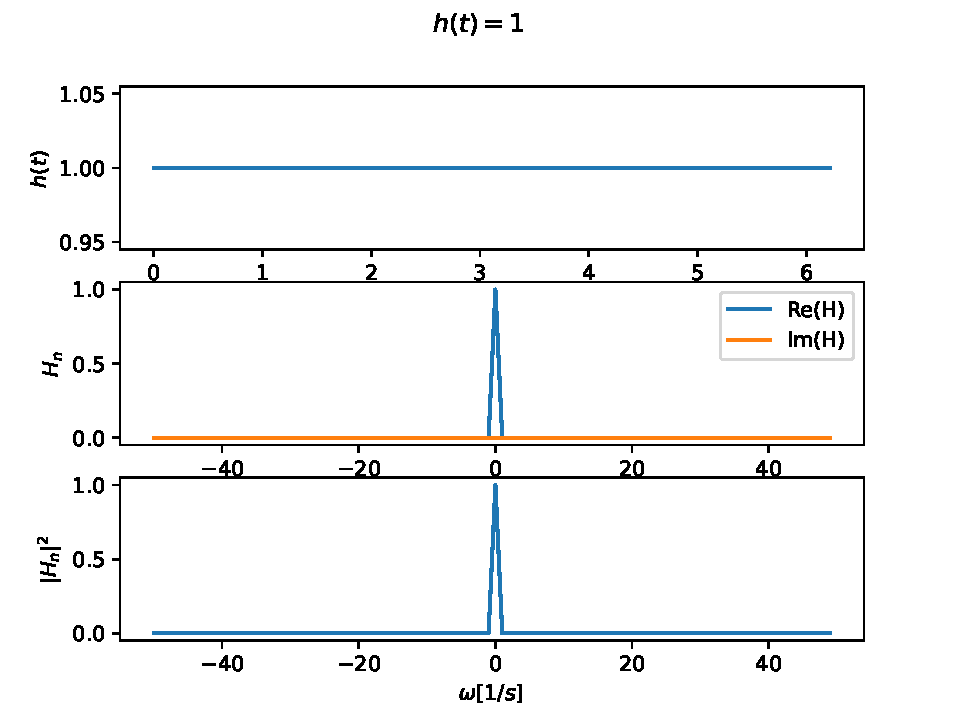
\includegraphics[width=\linewidth]{final_graphs/DFT_const.pdf}
  \caption{Fourier transfer of a constant function.} \label{fig:a}
  \end{subfigure}
  \hspace*{\fill}
  \begin{subfigure}{0.5\textwidth}
  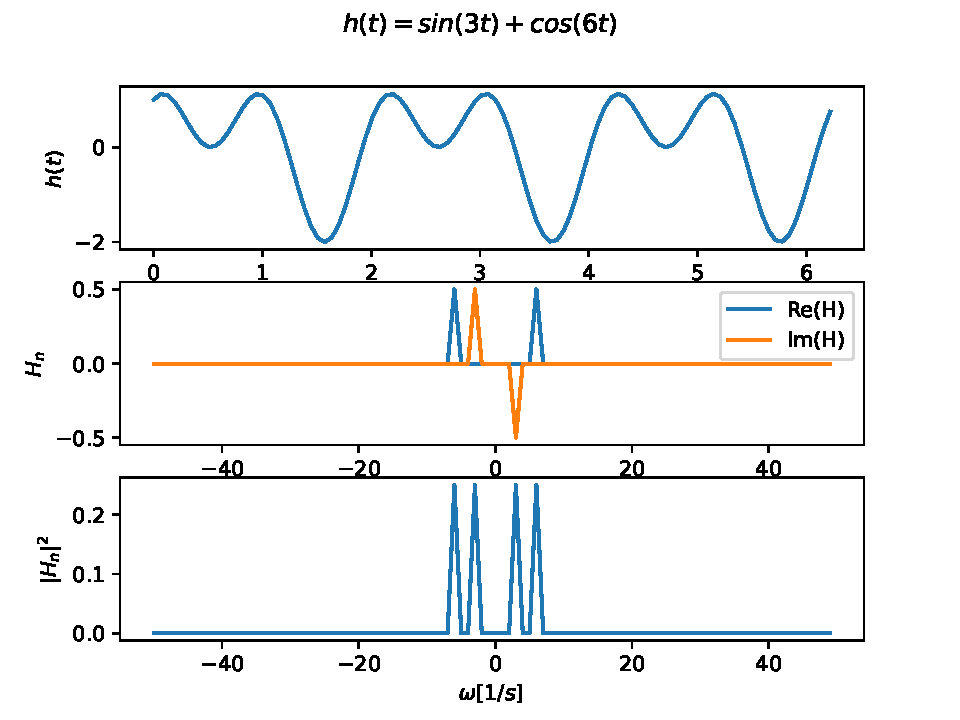
\includegraphics[width=\linewidth]{final_graphs/DFT_trig.pdf}
  \caption{Fourier transform of the sum of sine and cosine functions.} \label{fig:b}
  \end{subfigure}
  \medskip
  \begin{subfigure}{0.5\textwidth}
  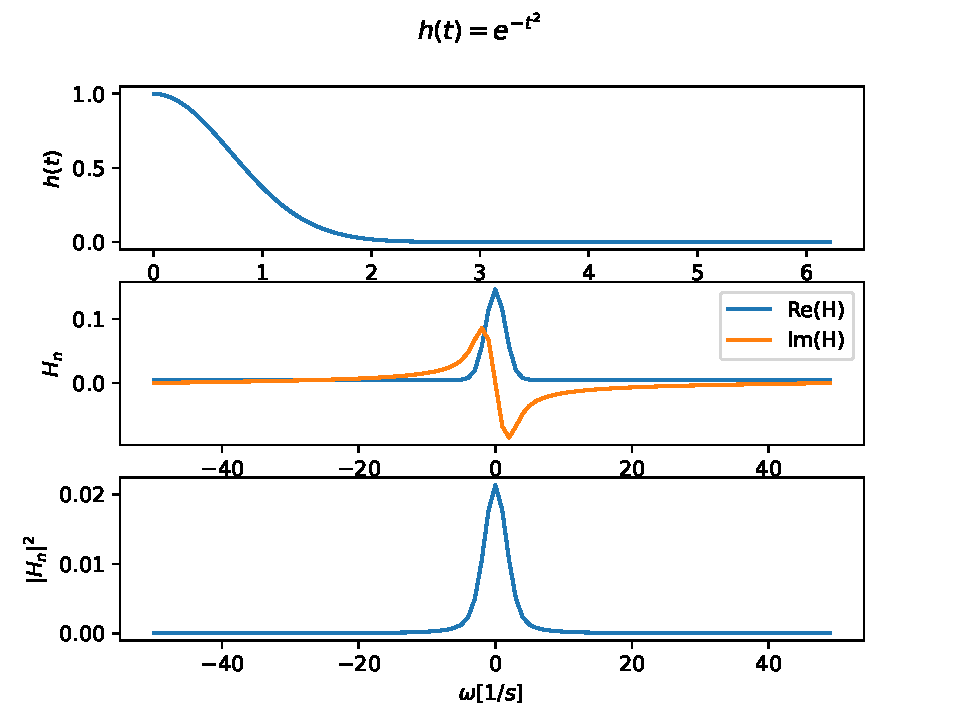
\includegraphics[width=\linewidth]{final_graphs/DFT_Gauss.pdf}
  \caption{Fourier transform of Gaussian function.} \label{fig:c}
  \end{subfigure}
  \hspace*{\fill}
  \begin{subfigure}{0.5\textwidth}
  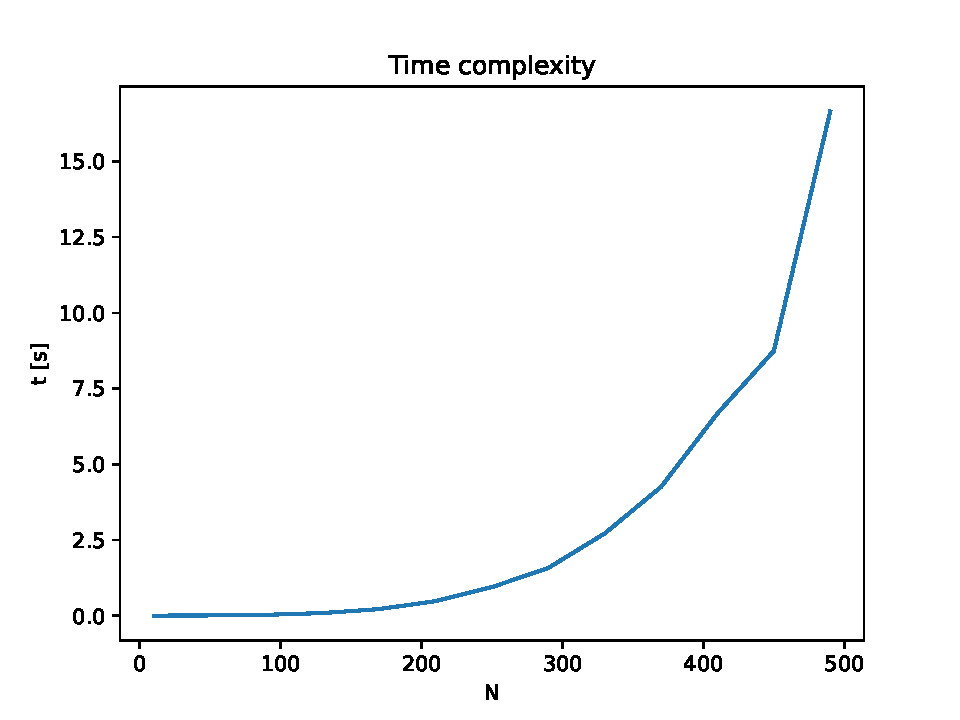
\includegraphics[width=\linewidth]{final_graphs/time_vs_N.pdf}
  \caption{Computation time in relation to the number of samples for all three methods.} \label{fig:d}
  \end{subfigure} 
  \caption{Implementation testing} \label{fig:1}
\end{figure}

We can compare the time complexity of each of the methods. The slowest one is the for loop implementation. This is a direct connection with the slow implementation of the for loop in Python. To circumvent the use of loops all the operations can be performed using vectors. This decreases the computation time by two magnitudes compared to for loop. The issue that arises with the use of vectors is memory usage. As we have to store all the data points in a vector of size $N$ and the algorithm generates a matrix of size $N \times N$, where the size of $N$ can quickly reach $10^6$ and above. When this happens most computers run out of memory, with $N=10^6$ you would need around $1 TB$ of storage to store the matrix. Memory issues don't arise in the for loop method as we generate the elements sequentially. Memory and timing constraints can be solved using fast Fourier transform which is six magnitudes faster than the vector method. Time complexity of all the methods is $O(n^2)$ as can be inferred from Figure 1d.

\section{Properties of Fourier transform}

Initial testing of the implemented Fourier transform was done using perfect data, following all the constraints set in the derivation. The first constraint we can break is sampling a signal that contains frequencies higher than the Nyquist criteria allows. First graph of Figure 2a shows the combination of a signal with higher and lower frequency compared to the sampling frequency. The blue line shows the correct input and the orange one the inverse transform of the Fourier transform. We can observe that the higher frequency details are lost. Looking at the power spectrum we can clearly observe two peaks at $5 Hz$ and $15 Hz$. The first one is correct whereas the second one is a mirror image of the $25 Hz$ part, $40 Hz - 25 Hz = 15 Hz$.

The second constraint is periodicity. If we transform a function that doesn't contain $n$ full periods, $n = 1, 2, \dots$, we observe a phenomenon called leakage. Comparing Figure 1b and 2b we can clearly see that the peaks in the power spectrum are wider as well as real and complex parts of the transform.

Both issues with constraints can solved using zero padding, where we add zeros to the end of out signal. Figure 2c presents a padded signal containing frequencies: 3, 8, and 30. We can clearly see all the three peaks which we wouldn't if there were not zeros. We can also observe the fast oscillations in the spectrum, which is an artefact of this methods.

We also implemented the inverse Fourier transform as it is presented in equation 4. Figure 2d examines the absolute error of the inverse and the input function for both implemented methods. The error remains below $10^{-13}$ which demonstrates the accuracy of the Fourier transform as well as the inverse.

\begin{figure}[hbtp]
  \begin{subfigure}{0.5\textwidth}
  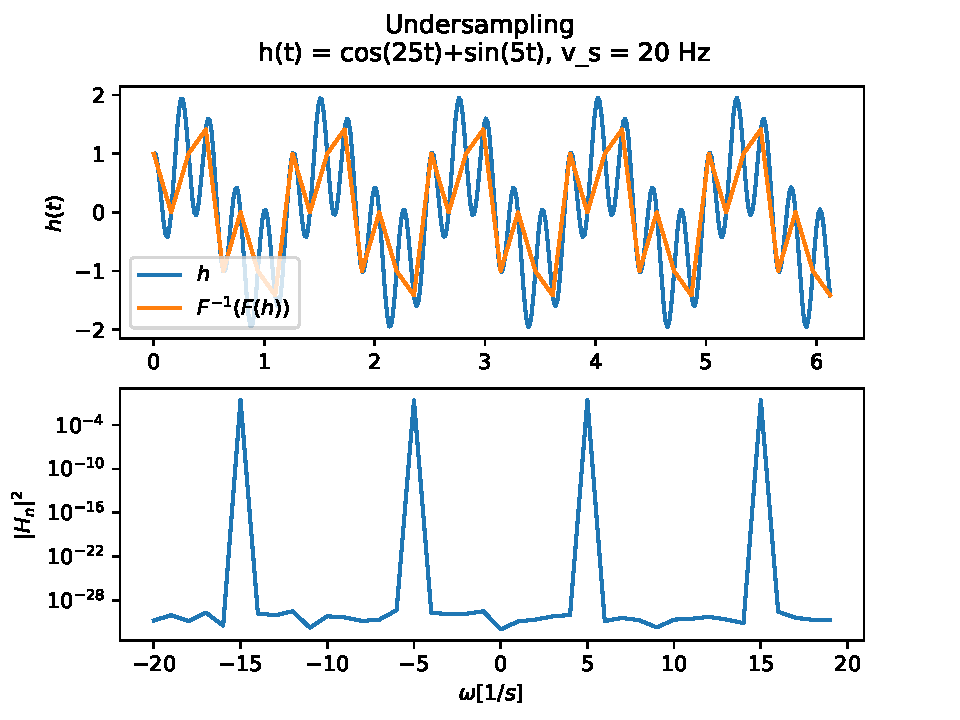
\includegraphics[width=\linewidth]{final_graphs/undersampling.pdf}
  \caption{Signal undersampling} \label{fig:a}
  \end{subfigure}
  \hspace*{\fill}
  \begin{subfigure}{0.5\textwidth}
  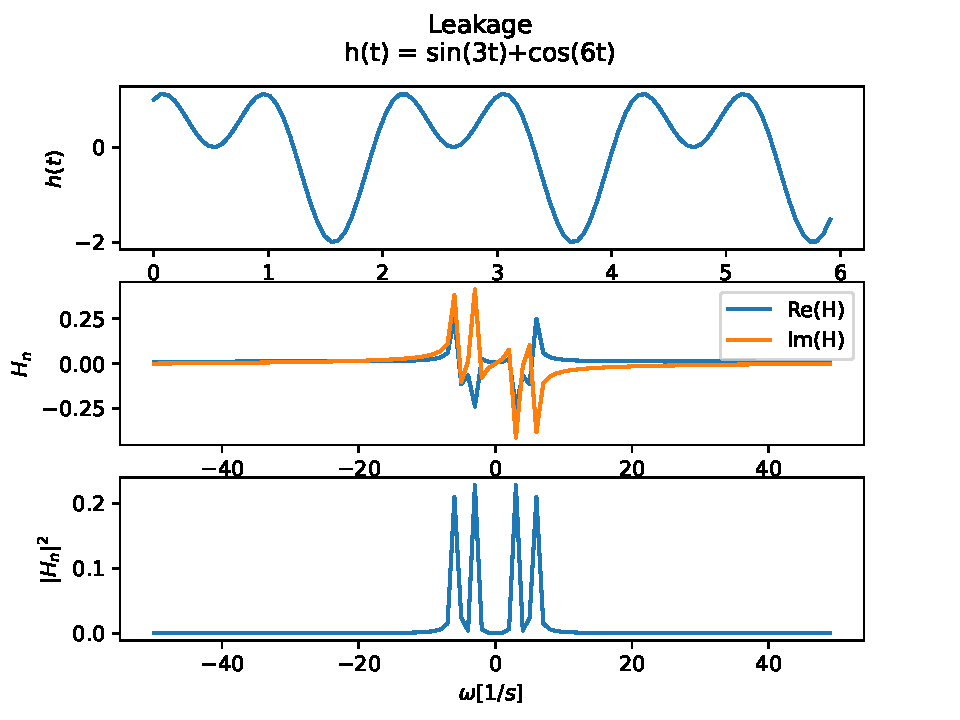
\includegraphics[width=\linewidth]{final_graphs/leakage.pdf}
  \caption{Leakage for non-periodic functions.} \label{fig:b}
  \end{subfigure}
  \medskip
  \begin{subfigure}{0.5\textwidth}
  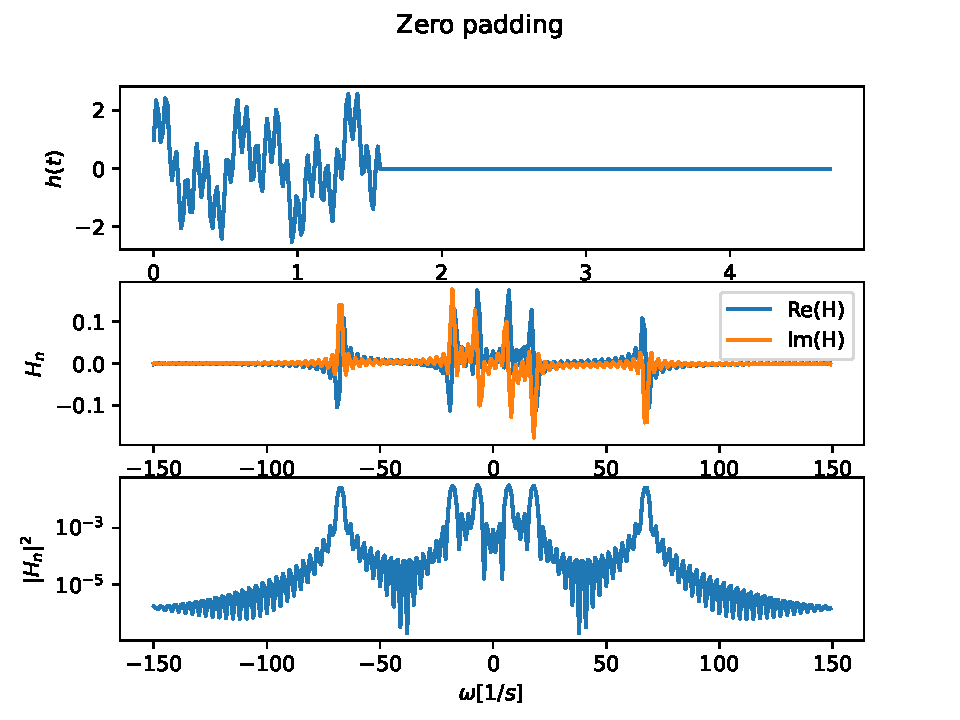
\includegraphics[width=\linewidth]{final_graphs/zero_padding.pdf}
  \caption{Zero padding method.} \label{fig:c}
  \end{subfigure}
  \hspace*{\fill}
  \begin{subfigure}{0.5\textwidth}
  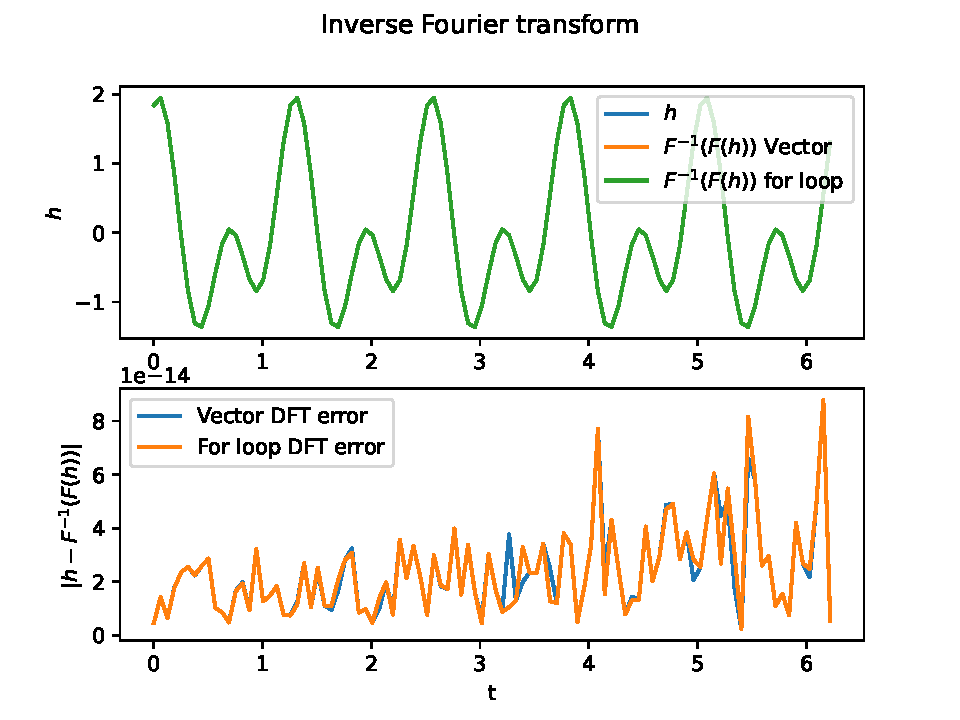
\includegraphics[width=\linewidth]{final_graphs/inverse.pdf}
  \caption{The accuracy of the inverse Fourier transform.} \label{fig:d}
  \end{subfigure} 
  \caption{Properties of Fourier transform.} \label{fig:1}
\end{figure}

\section{Music analysis}

In this section we performed the spectral analysis of the first three bars of a piece for violin called Violin partita No. 1 in B Minor by J. S. Bach. We compared different tracks sampled at consequently higher sampling frequencies, going from $882 Hz$ up to $44100 Hz$. Listening to the tracks we notice that the sound progressively becomes clearer and clearer. Observing the power spectrum we can see that by increasing the sampling frequency we start to hear higher frequencies.

To perform the transform we used Numpy FFT due to the large number of samples. The x axis also had to be scaled correctly. On the graph you can also see the notes performed in the piece. The majority of the peaks line up exactly with the lines.

\begin{figure}[hbtp]
  \begin{center}
  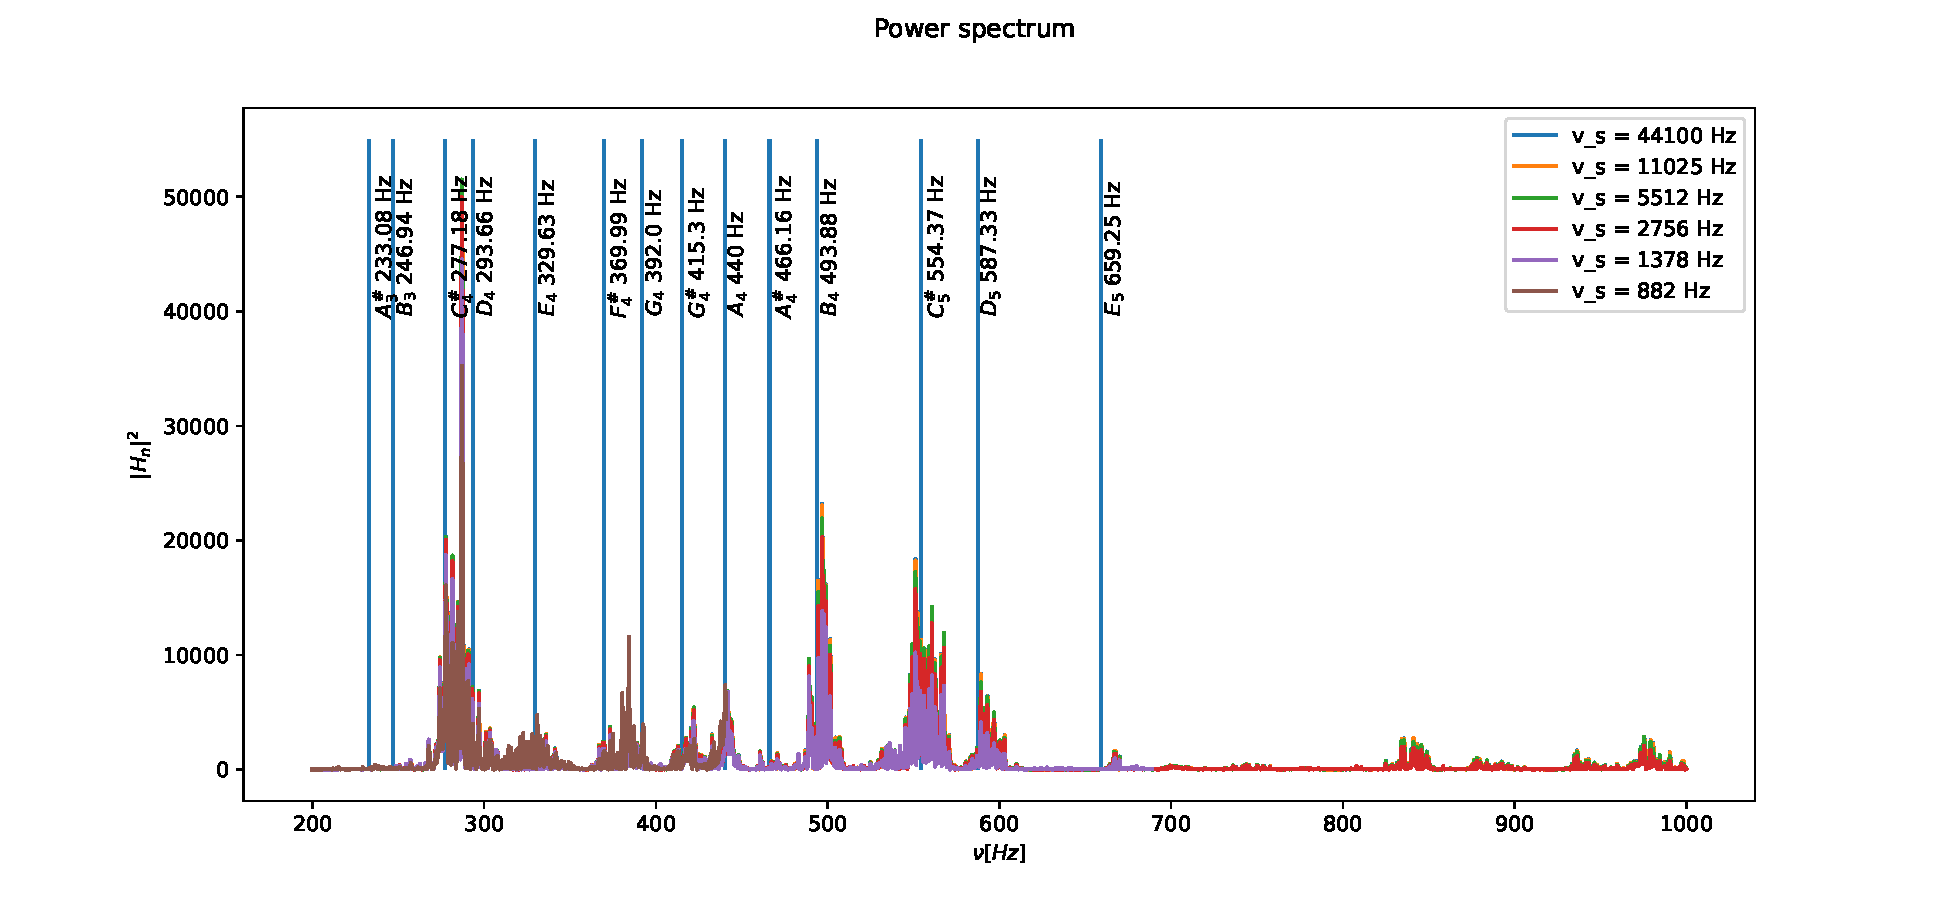
\includegraphics[width=\linewidth]{final_graphs/spectrum.pdf}
  \caption{Power spectrum of Bach Violin partita.}
  \end{center}
\end{figure}

\section{Stock market analysis}

For the extra part I decided to analyse the stock market. I took the opening price of S\&P 500 index fund going back 1 and 10 years. The S\&P 500 index is one of the best indicators of the state of the stock market. To get any useable data we first have to remove the linear upwards trend of the market. Now we are left only with oscillations from the mean. The power spectrum of these oscillations shows that only low frequencies are present in the data. Higher frequencies are uniformly distributed. Therefore we cannot find any patters on the daily or monthly scale, except on a multi-year scale. During research I found similar results published by other authors. Results are similar if we compare the 1 year and 10 year analysis.

\begin{figure}[hbtp]
  \begin{center}
  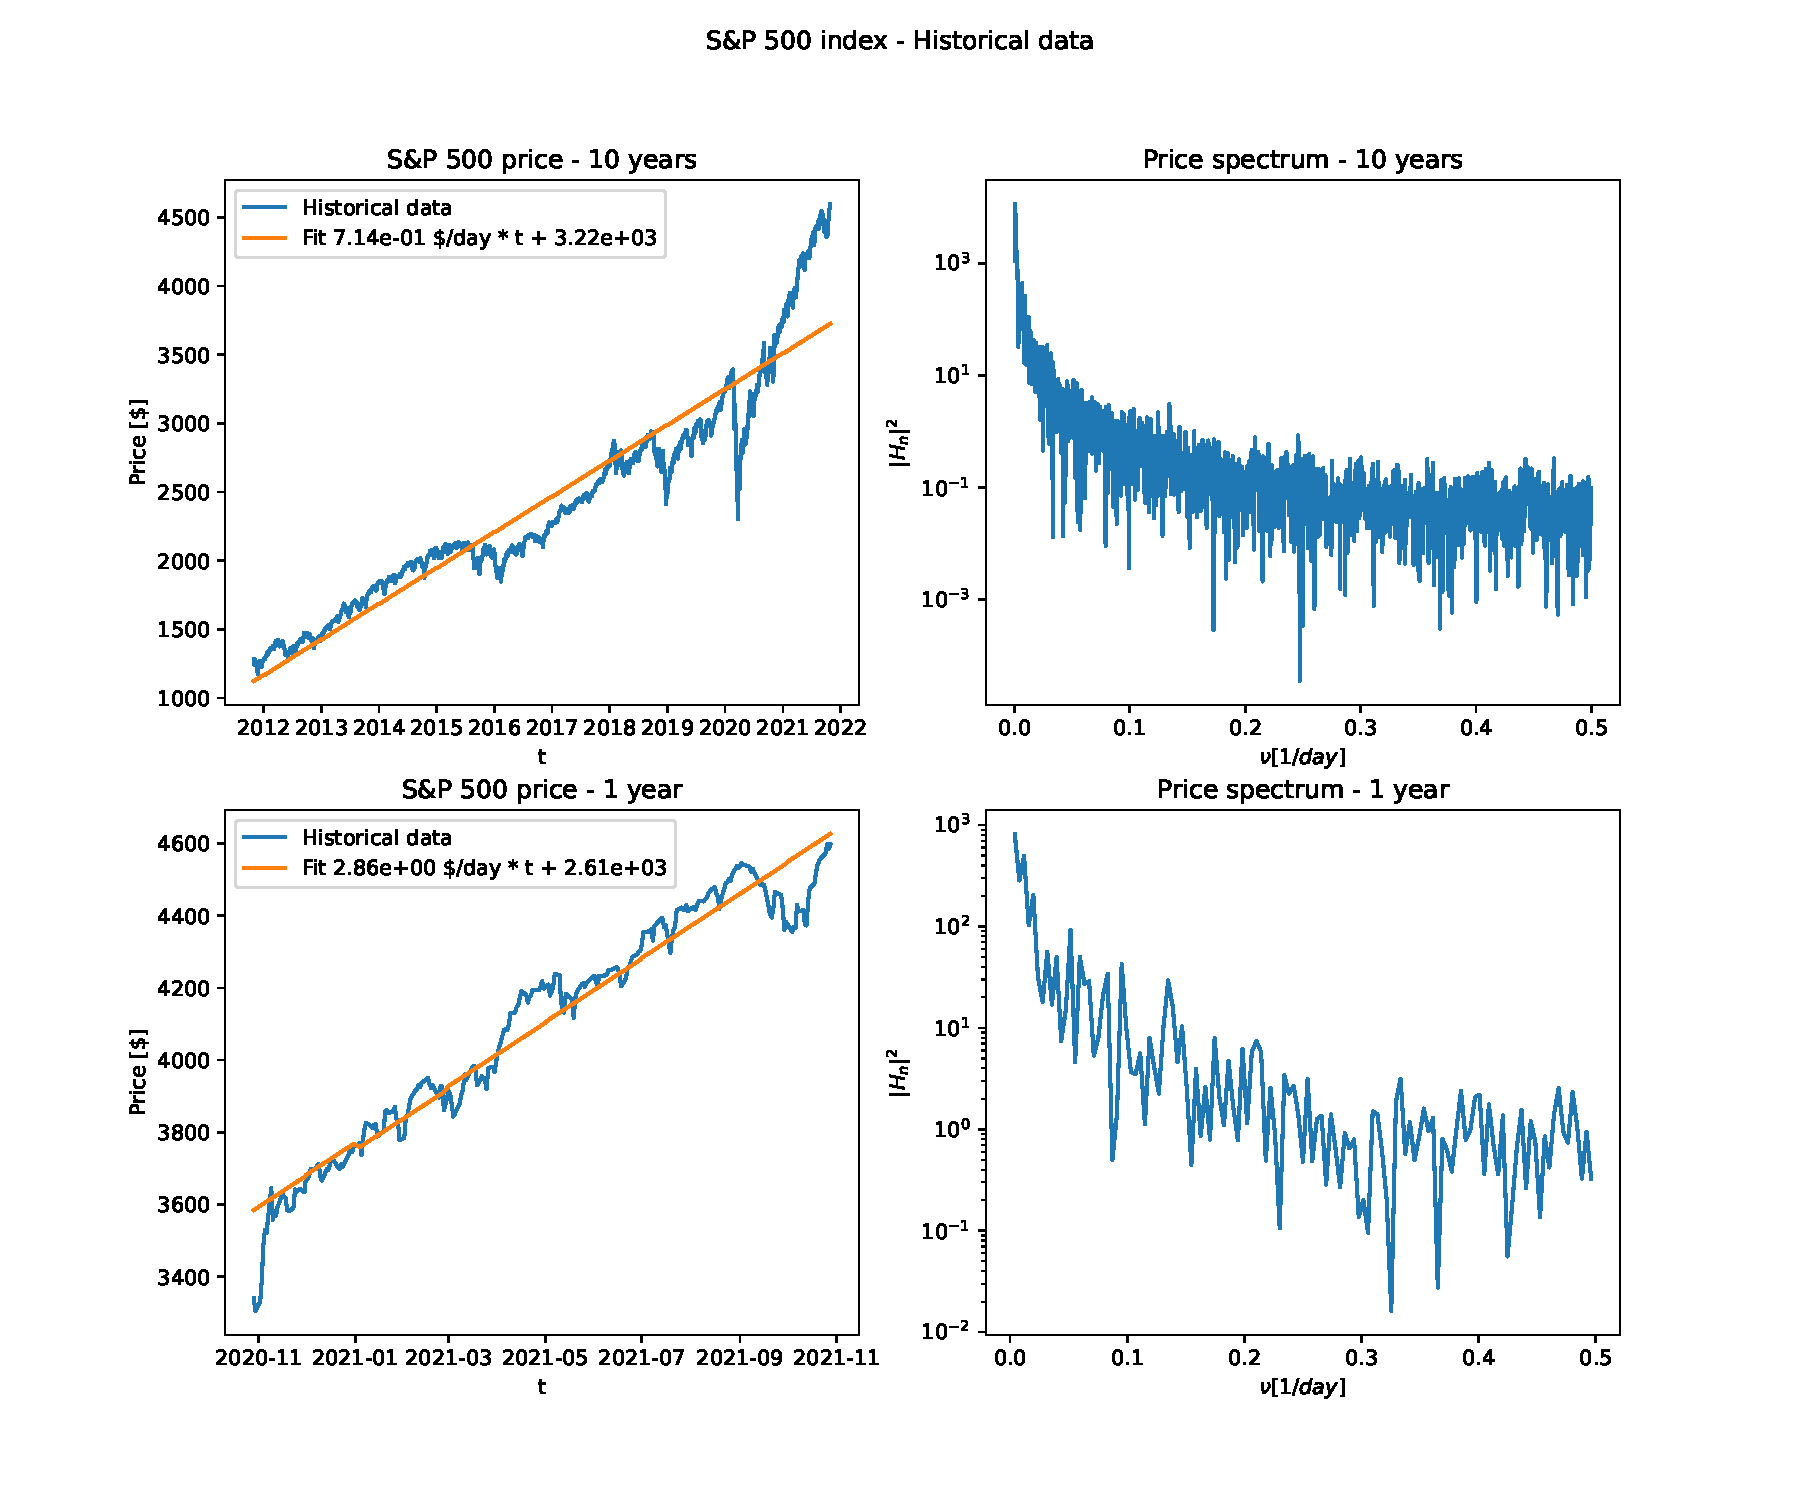
\includegraphics[width= \linewidth]{final_graphs/index.pdf}
  \caption{Fourier analysis of the stock market.}
  \end{center}
\end{figure}

\section{Conclusion}
The aim of this exercise was to analyst the Fourier transform and use it on different sets of data. We first showed how the transform works on simple functions and examined it's properties. Later we moved to real life data and analysed a song and the stock market.

\end{document}

